\subsection{Kürzester Weg}

\subsubsection*{Dijkstra}

\begin{figure}[h]
\centering
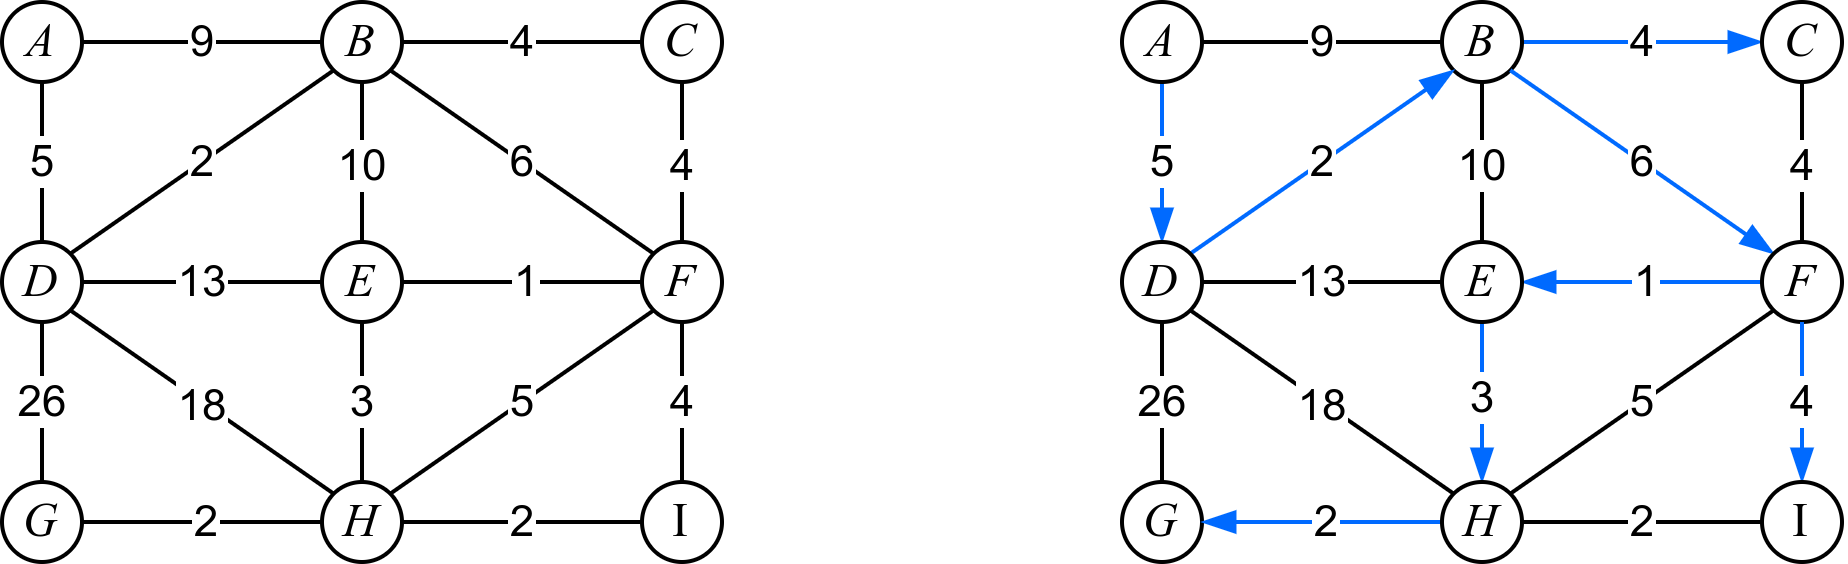
\includegraphics[width=0.9\textwidth]{graphics/dijkstra.png}
\end{figure}

\begin{table}[h]
\centering
\begin{tabular}{c|c|c|c|c|c|c|c|c||l}
A & B & C & D & E & F & G & H & I & S\\
\hline
0(A) &      & & & & & & & & A\\
0(A) & 9(A) &       & 5(D) & & & & & & A, D\\
0(A) & 7(D) &       & 5(D) & 18(E) & & 31(D) & 23(D) & & A, D, B\\
0(A) & 7(D) & 11(B) & 5(D) & 17(E) & 13(B) & 31(D) & 23(D) & & A, D, B, C\\
0(A) & 7(D) & 11(B) & 5(D) & 17(E) & 13(B) & 31(D) & 23(D) & & A, D, B, C, F\\
0(A) & 7(D) & 11(B) & 5(D) & 14(F) & 13(B) & 31(D) & 18(F) & 17(F) & A, D, B, C, F, E\\
0(A) & 7(D) & 11(B) & 5(D) & 14(F) & 13(B) & 31(D) & 17(E) & 17(F) & A, D, B, C, F, E, H\\
0(A) & 7(D) & 11(B) & 5(D) & 14(F) & 13(B) & 31(D) & 17(E) & 17(F) & A, D, B, C, F, E, H, I\\
0(A) & 7(D) & 11(B) & 5(D) & 14(F) & 13(B) & 31(D) & 17(E) & 17(F) & A, D, B, C, F, E, H, I, G
\end{tabular}
\end{table}

\begin{itemize}
\item Kann bei negativen Kanten ein falsches Ergebnis liefern, da er davon ausgeht, dass einmal besuchte Knoten nicht mehr verbessert werden können. Bei negativen Kanten ist dies jedoch möglich.
\item Bei negativen Kanten Gewichte deshalb lieber Bellman-Ford-Algorithmus
\end{itemize}

\newpage

\subsubsection*{Floyd}

\begin{figure}[h]
\centering
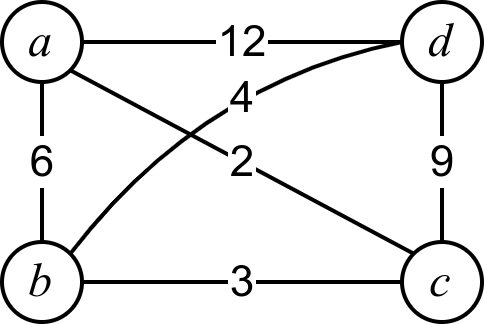
\includegraphics[width=0.3\textwidth]{graphics/floyd.png}
\end{figure}

\begin{table}[h]
\centering
\begin{tabular}{c|c|cccc|cccc}
& $i$ & $a$ & $b$ & $c$ & $d$ & $a$ & $b$ & $c$ & $d$\\
\hline
& $a$ & 0  & 6 & 2 & 12 & $a$ & $a$ & $a$ & $a$\\ 
& $b$ & 6  & 0 & 3 & 4  & $b$ & $b$ & $b$ & $b$\\
& $c$ & 2  & 3 & 0 & 9  & $c$ & $c$ & $c$ & $c$\\
& $d$ & 12 & 4 & 9 & 0  & $d$ & $d$ & $d$ & $d$\\
\hline
1 & $a$ & {\color{red}0}  & {\color{red}6} & {\color{red}2} & {\color{red}12} & {\color{red}$a$} & {\color{red}$a$} & {\color{red}$a$} & {\color{red}$a$}\\ 
1 & $b$ & {\color{red}6}  & 0 & 3 & 4  & $b$ & $b$ & $b$ & $b$\\
1 & $c$ & {\color{red}2}  & 3 & 0 & 9  & $c$ & $c$ & $c$ & $c$\\
1 & $d$ & {\color{red}12} & 4 & 9 & 0  & $d$ & $d$ & $d$ & $d$\\
\hline
2 & $a$ & 0  & {\color{red}6} & 2 & {\color{blue}10} & $a$ & $a$ & $a$ & {\color{blue}$b$}\\ 
2 & $b$ & {\color{red}6}  & {\color{red}0} & {\color{red}3} & {\color{red}4} & {\color{red}$b$} & {\color{red}$b$} & {\color{red}$b$} & {\color{red}$b$}\\
2 & $c$ & 2  & {\color{red}3} & 0 & {\color{blue}7}  & $c$ & $c$ & $c$ & {\color{blue}$b$}\\
2 & $d$ & {\color{blue}10} & {\color{red}4} & {\color{blue}7} & 0  & {\color{blue}$b$} & $d$ & {\color{blue}$b$} & $d$\\
\hline
3 & $a$ & 0  & {\color{blue}5} & {\color{red}2} & {\color{blue}9} & $a$ & {\color{blue}$c$} & $a$ & $b$\\
3 & $b$ & {\color{blue}5}  & 0 & {\color{red}3} & 4  & {\color{blue}c} & $b$ & $b$ & $b$\\
3 & $c$ & {\color{red}2}  & {\color{red}3} & {\color{red}0} & {\color{red}7}  & {\color{red}$c$} & {\color{red}$c$} & {\color{red}$c$} & {\color{red}$b$}\\
3 & $d$ & {\color{blue}9} & 4 & {\color{red}7} & 0  & {\color{blue}c} & $d$ & $b$ & $d$\\
\hline
4 & $a$ & 0 & 5 & 2 & {\color{red}9} & $a$ & $c$ & $a$ & $b$\\ 
4 & $b$ & 5 & 0 & 3 & {\color{red}4} & $c$ & $b$ & $b$ & $b$\\
4 & $c$ & 2 & 3 & 0 & {\color{red}7} & $c$ & $c$ & $c$ & $b$\\
4 & $d$ & {\color{red}9} & {\color{red}4} & {\color{red}7} & {\color{red}0} & {\color{red}$c$} & {\color{red}$d$} & {\color{red}$b$} & {\color{red}$d$}\\
\end{tabular}
\end{table}

\newpage

\subsubsection*{FIFO}

\begin{figure}[h]
\centering
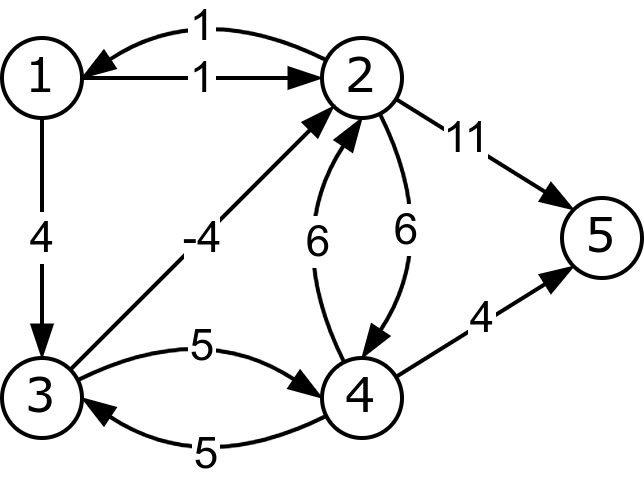
\includegraphics[width=0.35\textwidth]{graphics/fifo.png}
\end{figure}

\begin{table}[h]
\centering
\begin{tabular}{c|c|c|c|c||c|c|c|c|c||l}
D(s,1) & D(s,2) & D(s,3) & D(s,4) & D(s,5) & R(1) & R(2) & R(3) & R(4) & R(5) & S\\
\hline
0 &   &   &   &    & &   &   &   &   & $1$\\
0 & 1 & 4 &   &    & & 1 & 1 &   &   & $2 < 3$\\
0 & 1 & 4 & 7 & 12 & & 1 & 1 & 2 & 2 & $3 < 4 < 5$\\
0 & 0 & 4 & 7 & 12 & & 3 & 1 & 2 & 2 & $4 < 5 < 2$\\
0 & 0 & 4 & 6 & 11 & & 3 & 1 & 2 & 4 & $5 < 2$\\
0 & 0 & 4 & 6 & 11 & & 3 & 1 & 2 & 4 & $2$\\
0 & 0 & 4 & 6 & 10 & & 3 & 1 & 2 & 4 & $4$\\
0 & 0 & 4 & 6 & 10 & & 3 & 1 & 2 & 4 & $5$\\
0 & 0 & 4 & 6 & 10 & & 3 & 1 & 2 & 4 &
\end{tabular}
\end{table}
